
% this file is called up by thesis.tex
% content in this file will be fed into the main document

%: ----------------------- introduction file header -----------------------
\begin{savequote}[50mm]
Personally, I think it does help, that it makes a beneficial difference, but the scientific literature on the subject is very messy.
\qauthor{Jeanne Petrek}
%“And upon the top of the pillars was lily work: so was the work of the pillars finished.”
%
% Bible quotes
\end{savequote}


\section{User Modelling}
\label{sec:user}

% the code below specifies where the figures are stored
\ifpdf
    \graphicspath{{2_state_of_the_art/figures/PNG/}{2_state_of_the_art/figures/PDF/}{2_state_of_the_art/figures/}}
\else
    \graphicspath{{2_state_of_the_art/figures/EPS/}{2_state_of_the_art/figures/}}
\fi


%------------------------------------------------------------------------- 

\subsection{A Chronological Review of the Evolution of User Models}
\label{sec:chronological_review}

The following figure illustrates the evolution and different solutions by 
chronological order for the last 15 years. During these years different user
characteristics have been taken into account considering the final purpose of
the designed system. 

\vspace{1cm}
\setlength\taskwidth{1.7cm}

\begin{timeline}
  \label{chr:users}
  \Task[1991]{\citet{orwant_doppelgangeruser_1991}}
  \Task[1994]{\citet{brajnik1994shell}, \citet{paiva1994tagus}, \citet{kay1994toolkit}}
  \Task[1999]{\citet{pohl_logic_based_1999}}
  \Task[2001]{\citet{fischer_user_2001}, \citet{kobsa_generic_2001}.}
  \Task[2002]{\citet{gregor_designing_2002}}
  \Task[2003]{\citet{gauch_ontology_based_2003}, \citet{razmerita_ontology_based_2003}}
  \Task[2005]{\citet{hatala_ontology_based_2005}, \citet{pereira_triple_2005}, \citet{heckmann_gumogeneral_2005}}
  \Task[2007]{\citet{persad_characterising_2007}, \citet{golemati_creating_2007}}
  \Task[2008]{\citet{casas_user_2008}}
  \Task[2012]{\citet{evers_achieving_2012}, \citet{skillen2012ontological}}
\end{timeline}


First user modelling systems started in the late eighties. 
\citet{allen_plan_based_1979},~\citet{cohen_elements_1979}, 
~\citet{perrault_speech_1978},~\citet{rich_building_1979} 
and~\citep{rich_user_1979} are examples of researchers whose works inspired next 
user modelling approaches. From there several authors started collecting 
different types of information about the users and exhibiting, for example, 
different kinds of adaptations to them~\citep{kobsa_generic_2001}.

Before overview the evolution, a definition of user modelling is needed. There 
are at least two different perspectives which might answer this question. One of 
these is related to the \ac{ai} research area, and it considers user modelling 
as the process through which systems gather information and knowledge about 
users and their individual characteristics. Therefore, a user model is considered 
a source of information about the user of the system which contains several
assumptions about several relevant behaviour or adaptation data. However, in
this thesis the \ac{hci} research perspective is taken, which is defined by
\citet{pohl_logic_based_1999} as follows:

\begin{description}
  \item[\Defi{User Model, by \citet{pohl_logic_based_1999}}] \hfill \\
  \begin{mdframed}[hidealllines=true,backgroundcolor=gray!20]
  \textit{``It refers to an a-priori model of the users of a computer system that the system
  designer has in mind, or to the assumed models that users will probably develop
  of the system and the tasks they can perform using the system''}~\citep{pohl_logic_based_1999}.
  \end{mdframed}
\end{description}

Nevertheless, this definition and the \ac{ai} perspective coincide in the idea that 
every system must use information about the user to be able to see and react to 
their different problems and needs and improve the system purpose. This section 
analyses the most significant user models in the past 15 years.

\subsection{User models}
\label{sec:user_models}

%sota user models
\subsubsection{1991: Jon Orwan and the Doppelgänger system}
\label{sec:orwant_doppelganger}

Doppelgänger is a user modelling system that performs inferences upon user data
and makes this information available to applications. The system allows users to
modify their models, it makes implicit generalizations about the data (which is
gathered through different channels) and provides an extensible architecture~\citep{orwant_doppelgangeruser_1991}. 

% ``Figure 1 The DOPPELGÄNGER user modelling system gathers data about users from sensors, makes inferences on
% those data, and makes the results available to applications'' cogido de http://www.cs.ucf.edu/~dcm/Teaching/COT4810-Spring2011/Presentations/FrankHines-CheapUserModelingForAdaptiveSystems.pdf

User data is gathered through a continuously operative sensor network which
senses users' everyday activities (see Listing~\ref{lst:orwant_sensor_1}). Hence,
both long-term and short-term information about the user are stored. Sensors are
integrated in users' activities. However, Doppelgänger acknowledges the imperfection
of real world data. Data streams are usually incomplete or erroneous. The main
objective of the Doppelgänger system is to recover from these imperfections through
several learning techniques:

\begin{itemize}
  \item The Beta distribution~\citep{drake_fundamentals_1967}, which is used to
  determine the preference strength, probability of accuracy and the confidence
  of an estimation.
  \item Linear prediction, to predict a possible next event.
  \item Markov models, which represents user's behaviour through several states and
  all possible transitions between them with the corresponding probability.
\end{itemize}


The system maintains an accuracy estimation for each sensor, which helps the
system to decide a confidence metric for the gathered data.

\begin{minted}[linenos=true, fontsize=\footnotesize, frame=lines]{json}
(object orwant location (place 344) (time 779562701) 
(id active-badge))
\end{minted}
\captionof{listing}{Message from a sensor to the server~\citep{orwant_heterogeneous_1994}.\label{lst:orwant_sensor_1}}


The user models are represented in SPONGE, a LISP based data structure manipulated with
C and Pearl programs \citep{orwant_heterogeneous_1994} (see Listing~\ref{lst:orwant_sensor_2}). 
Models are stored as Unix directories consisting of domain submodels and conditional 
submodels. The first one contains information about the user behaviour (i.e., 
location, preferences, and so forth); the second group contains triggering information 
for deciding actions when certain situations are met. Besides, each user model 
is conceptually represented as a point in a high dimensional space in which the 
dimensions are determined by the number of sensors in the network.


% \InsertFig{orwant}{fig:orwant}{Orwant user model \citep{orwant_heterogeneous_1994}}{}{0.70}{}
% 
% \InsertFig{orwant}{fig:orwant_sensors_apps}{The DOPPELGÄNGER user modelling system gathers data about users from sensors, makes inferences on
% those data, and makes the results available to applications. \citep{orwant_for_1996}}{}{0.70}{}

\begin{minted}[linenos=true, fontsize=\footnotesize, frame=lines]{json}
(object orwant primary
  (object biographical_data
    (string_binding "true name" "Jon Orwant")
    (string_binding "e-mail address" orwant@media.mit.edu)
  ...)
  (object control
    (int_binding "doppelganger ID" 4))
...)
\end{minted}
\captionof{listing}{Orwant user model~\citep{orwant_heterogeneous_1994}.\label{lst:orwant_sensor_2}}

% \begin{figure}
% \centering
% \includegraphics[width=0.7\textwidth]{orwant_sensors_apps.pdf}
% \caption{The DOPPELGÄNGER user modelling system gathers data about users from sensors, makes inferences on
% those data, and makes the results available to applications~\citep{orwant_for_1996}.}
% \label{fig:orwant_sensors_apps}
% \end{figure}
% ----------------------------------------------------------------------


\subsubsection{2001: Gerhard Fischer}
\label{sec:fischer_user_2001}

In 2001~\citet{fischer_user_2001} reviews the user models of the past 10 years. 
He describes how using computers in \ac{hci} environments has been always
modelled as a user-computer couple. These elements are modelled as an explicit 
connection which represents the communication between them. New and modern 
interfaces such as windows, menus, pointers, colours, sound and touch screens 
have enlarged this communication line thanks to their capabilities.

Furthermore, in addition to the possibilities of new design approaches,
knowledge-based architectures in \ac{hci} explore the possibility of implicit
communication channel. The required knowledge considers the problem domain,
communication processes and the communication agent. Users are part of the
communication agent group. Fischer defends the idea that there are many types of
users. Besides, their needs change with the experience and through time.
Hence, a simple user classifications (e.g., \textit{novel}, \textit{intermediate}
and \textit{expert}) is not enough to characterize users in complex environments. 
Nevertheless, despite Fischer remarks the significance of each agent, he does 
not establish which agent capabilities are important to face the problem of 
modelling a user.

% \InsertFig{fischer}{fig:fischer}{The human-computer interaction channel 
% \citep{fischer_user_2001}}{}{0.70}{}

\begin{figure}
\centering
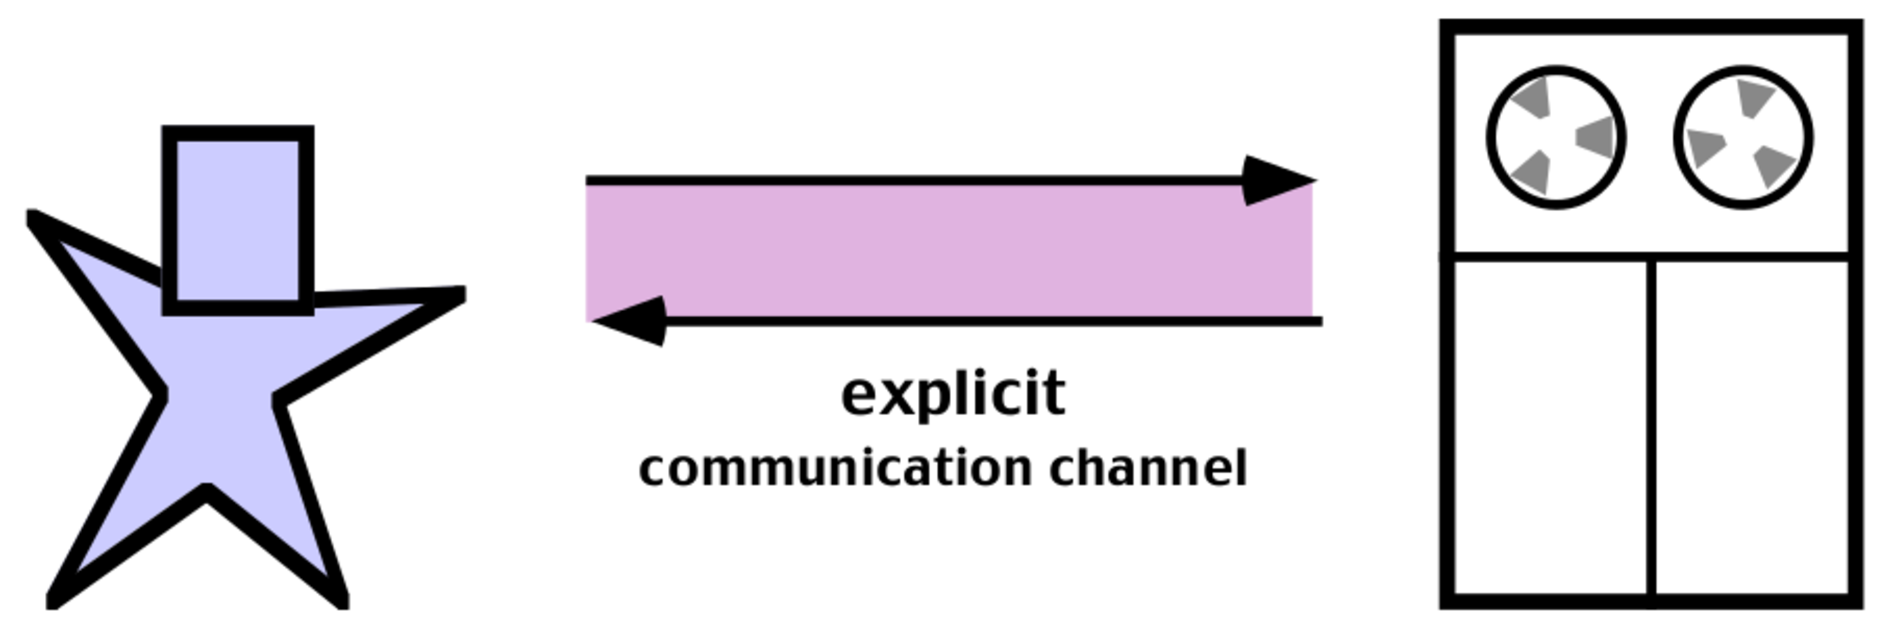
\includegraphics[width=0.50\textwidth]{fischer.pdf}
\caption{The \ac{hci} channel~\citep{fischer_user_2001}.}
\label{fig:fischer}
\end{figure}
\subsubsection{2002: Gregor et al.}
\label{sec:gregor}

%------------------------------------------------------------------------- 
In 2002,~\citet{gregor_designing_2002} focus their approach on a certain groups 
of users: the elderly. A three group classification is presented. In the first 
group there are the fit older people, who do not suffer from any disability. The 
second group is formed by older fragile people who have one or more 
disabilities. Finally, the last group encompasses the older and people with 
disabilities whose capabilities to function depend on other people. In this 
case, the authors identify several user capabilities:

\begin{itemize}
 \item Physical, sensory and cognitive capabilities.
 \item The ability to learn new techniques (cognitive).
 \item Memory problems (cognitive).
 \item The environment can affect several elderly capabilities.
 \item Elderly experience (as a positive fact).
\end{itemize}

On the other hand,~\citet{gregor_designing_2002} consider that, as people grow 
older, their capabilities change. This process encompasses a reduction of 
cognitive, physical and sensory functions depending on the individual. This 
diversity is a significant issue for modelling users and designing computing 
systems.

Figure~\ref{fig:gregor} shows an adaptable user interface which takes into 
account these capabilities. 

% \InsertFig{gregor}{fig:gregor}{Adaptable browsing 
% interface~\citep{gregor_designing_2002}}{}{0.70}{}

\begin{figure}
\centering
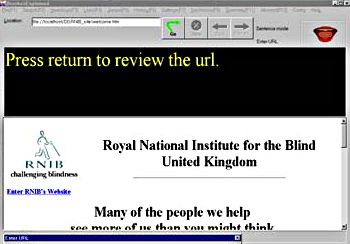
\includegraphics[width=0.70\textwidth]{gregor.png}
\caption{Adaptable browsing 
interface~\citep{gregor_designing_2002}.}
\label{fig:gregor}
\end{figure}

\subsubsection{2003: Gauch et al.}
\label{sec:gauch}

Towards the goal of personalized navigation of online information~\citet{gauch_ontology_based_2003}
provide a user ontology for dynamically modelling the user browsing. The ontology
is formed by several concepts which are weighted indicating the user's perceived
interest in the corresponding concept. These concepts are related with surfing
experience (i.e., the content, length and time spent) on each Web page and
classified into the reference ontology. Hence, the user profile is created 
automatically. This means that the user profile information is collected 
implicitly without user feedback, as the ontology's concepts are automatically 
weighted considering the amount of related information from the user browsing.


% ----------------------------------------------------------------------

\subsubsection{2003: Razmerita et al.: The OntobUM Ontology}
\label{sec:razmerita2003ontology}

Focused in the context of \ac{kms}~\citet{razmerita_ontology_based_2003} present
OntobUM, a generic ontology-based architecture for user modelling. The model is 
generated through two different ways:

\begin{itemize}
  \item Explicitly, using a user profile editor. Thus, the user has to 
  provide some information.
  \item Implicitly, information maintained by several intelligent services 
  which maintain and update the information about the user considering the 
  user's behaviour with the services and provide adapted services based on 
  user's preferences.
\end{itemize}

The architecture of the presented ontology is composed of the following ontologies:

\begin{itemize}
  \item The User Ontology, which structures the different characteristics and 
  preferences of the user.
  \item The Domain Ontology, which defines several concepts about the domain.
  \item The Log Ontology, which manages the semantics of the interaction 
  between the user and the whole system.
\end{itemize}

Authors identify several users' characteristics that are relevant for a \ac{kms} 
under the Behaviour concept. Nevertheless, most of the user ontology is 
generic and it is available to be used in other application domains. 

%Dynamic user modeling? Atención al proceso de captura de datos implícita.

\subsubsection{2005: Hatala and Wakary and the Ec(h)o system}
\label{sec:hatala}

Ec(h)o is an ontology-based augmented audio reality system for museums which 
aims to maintain rich and adaptive output information. The main purpose of this 
work is to address the problem of supporting experience design and functionality 
related to museum visits through user models combined with augmented reality 
and tangible user interface system.~\citet{hatala_ontology_based_2005} find
several challenges for capturing rich context information. For the presented 
museum scenario, social, cultural, historical and psychological factors are 
significant for the user experience. In this field, the argumentation made by
is remarked as relevant. \citeauthor{dourish_what_2004} states that activities 
and context are directly and dynamically linked \citet{dourish_what_2004}\citep{dourish_where_2004}.
This concept is called \textit{embodied interaction}.

The core of the ec(h)o's reasoning module is a dynamically updated user model
\citep{wahlster1989user}. The ruled-based model changes as the user moves 
through the museum and selects several audio objects. This models enables 
developers to consider which inputs influence user interests. In the ec(h)o 
system there are two ways of updating the model: the user movement and a 
selection of an audio object. These actions have different effects on the model 
of the user interests (i.e., influence of initial interest selection, of object 
selection on user interest and of location change). 

As it occurs with recommender systems, user's interest are vital for the concept
ontology. These concepts are weighted in the ontology as concepts which represent
the user's likes within the environment. Besides, an interaction history is 
maintained recording the way the user interacts with the museum. In addition to 
these characteristics the user type is also considered. Hence, the system is 
allowed to characterize the user experience with the environment. It classifies 
users into three different categories:

\begin{itemize}
  \item The \textit{avaricious} visitor, who wants to see as much as possible
  in a sequentially way.
  \item The \textit{selective} visitor, who is more selective with the concepts 
  he/she is interested in.
  \item The \textit{busy} visitor, who prefers to not spend much time and get a 
  general vision of the exhibition.
\end{itemize}

\subsubsection{2005: Fernando Pereira}
\label{sec:pereira}

Within a video adaptation and quality of experience evaluation scenario,
~\citet{pereira_triple_2005} studies a user characterization through three
different dimensions: sensory, perceptual and emotional. First of all,
\citeauthor{pereira_triple_2005} establishes the difference between sensations 
and perceptions as follows:

\begin{itemize}
  \item \textit{Sensations} are monomodal, more low-level, physical and less 
  related to the real world composition than perceptions. They regard the simple 
  conscious experience for the corresponding physical stimulus (e.g., light 
  variation and eyes reaction to this change). They are related to the first 
  contact between a human and the surrounding environment.
  
  \item \textit{Perceptions} are multimodal, and they are part of the cognition 
  process (knowing and learning) and regard the conscious experience and 
  identification of objects.
\end{itemize}

On the other hand, emotions are considered as central in a communication and 
entertainment process. Therefore, \citeauthor{pereira_triple_2005} proposes a 
triple layered \ac{spe} user model for the evaluation of the quality of 
experience in the consumption of multimedia content.





\subsubsection{2007: Heckmann et al.}
\label{sec:heckmann}

A different approach is implemented by~\citet{heckmann_gumogeneral_2005}.
Divided into four main groups (emotional state, personality, characteristics and
physiological state), the authors present the \acf{gumo}, an ontology model to 
characterize users capabilities within adaptive environments. A significant 
user aspect that is taken into account in this work is the stress. In the 
adaptive interfaces domain it is needed to pay special attention to the 
consequences of each adaptation. But the stress is not only determined  by this 
process. It is also derived from several user experiences, as the current 
context state (e.g. traffic, noise, surrounding people, and so 
forth~\citep{babisch_noise_stress_2002}). Figure~\ref{fig:heckmann_model} illustrates
the model presented by~\citeauthor{heckmann_gumogeneral_2005}.

% \InsertFig{heckmann_model}{fig:heckmann_model}{Several user model property
% dimensions~\citep{heckmann_gumogeneral_2005}}{}{0.70}{}

\begin{figure}
\centering
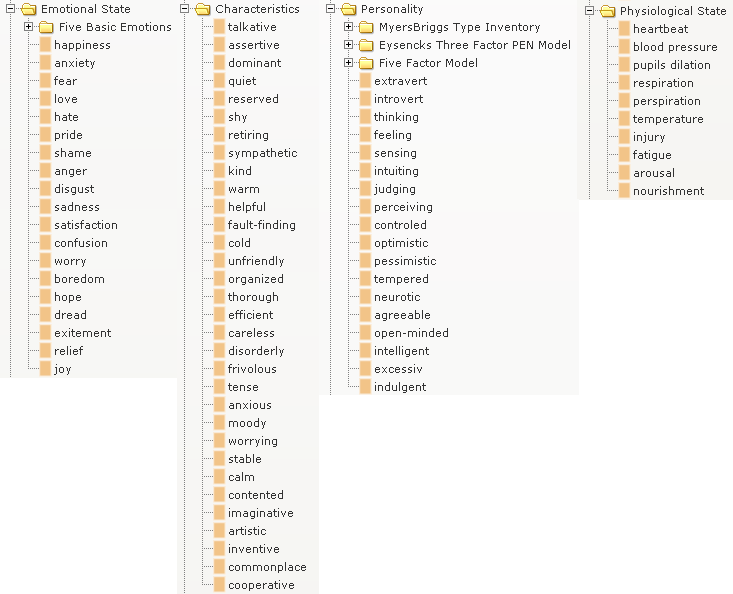
\includegraphics[width=0.70\textwidth]{heckmann_model.png}
\caption{Several user model property
dimensions~\citep{heckmann_gumogeneral_2005}.}
\label{fig:heckmann_model}
\end{figure}

% ----------------------------------------------------------------------

\subsubsection{2007: Persad et al.}
\label{sec:persad}

\citet{persad_cognitive_2007}\citep{persad_characterising_2007} relate user
capabilities and product demands as a tool to evaluate the product design (see Section~\ref{sec:motivation}).
\citeauthor{persad_characterising_2007} remark four main components to consider 
when dealing with interaction between people and technology: the user, the 
product, the environment or context, and the set of activities or tasks 
that define the interaction. The authors try to assess an adaptation degree 
between users and the designed products using different compatibility measures. 
These measures can be assessed on different levels of human capabilities, 
including sensory, cognitive and motor. The concepts of user capability and 
product demand provide a useful framework for analysing the user-device 
compatibility. The product demand levels are considered multidimensional and 
they are set by the interface attributes of the product itself. For example, 
a product's text display will be designed with a certain text size, font, and 
colour contrast. The combination of these attributes define the visual demand 
level within the user visual capabilities. Similarly, other combinations of 
product attributes command several cognitive and motor demands. 

\citeauthor{persad_cognitive_2007} also reviewed functional classifications 
and experimental studies to identify the most relevant low-level skills for 
designing products within the cognitive, motor and sensory domain. This is 
highly related to the \ac{icf} functions described in Section~\ref{sec:background_icf}.

\paragraph*{Sensory capabilities}
\subparagraph*{Visual capabilities:} Several sensory capabilities are known to 
deteriorate with ageing~\citep{persad_exploring_2006}. Thus, 
\citeauthor{persad_exploring_2006} state that the following functions seem to 
account for most of visual disability:

\begin{itemize}
  \item Visual acuity.
  \item Contrast sensitivity.
  \item Colour perception.
  \item Useful field of view.
  \item Stereopsis.
\end{itemize}


\subparagraph*{Hearing capabilities:} Loss of hearing capabilities may directly 
affect the speech interaction with the device. The main low-level hearing 
functions to guarantee the interaction are the following:

\begin{itemize}
  \item Pure tone detection thresholds.
  \item Speech detection and recognition discrimination thresholds.
  \item Sound localization.
\end{itemize}

% \subparagraph*{Environmental effects}
% The level of illumination, noise, weather, etc. are several environment features 
% which might affect user capabilities.

\paragraph*{Cognitive capabilities}
The product's user interface must be usable and accessible enough to guarantee 
that users easily understand the interaction. The following capabilities are 
related to the human cognitive domain:

\begin{itemize}
 \item Working memory performance.
 \item Long term memory.
 \item Mental models, planning and problem solving.
 \item Language and communication capabilities.
\end{itemize}

\paragraph*{Motor capabilities}
\subparagraph*{Upper limb capabilities:}
There are many conditions that affect manipulating a product (e.g., arthritis, 
stroke, multiple sclerosis, head injury, cerebral palsy and missing or damaged 
limbs). These problems directly reduce grasp forces, range of motion and fatigue 
thresholds~\cite{persad_characterising_2007}.

The following areas are highlighted within motor capabilities:
\begin{itemize}
  \item Reach ranges for each arm.
  \item Grasping, dexterity and force exertion.
  \item Two handed actions and coordination.
\end{itemize}

\subparagraph*{Gross body movement capabilities:}
Usually products require certain user mobility degree. 

\bigskip

Besides, \citeauthor{persad_characterising_2007} provide six general categories 
for product features and their interface classification. For this classification 
their toaster case study is considered, \textit{``which is used to demonstrate 
the capability-demand interaction''} (see Table~\ref{tbl:persad_product_interface}).

\begin{table}
  \caption{Product interface classification by~\citet{persad_characterising_2007}.}
  \label{tbl:persad_product_interface}
\footnotesize
\centering
    \begin{tabular}{l l}
    \hline
    \textbf{Feature type} 	& \textbf{Examples} \\
    \hline
    Product chassis 		& Handles, gripping surface. 		\\
    Displays and indicators 	& Visual and auditory displays. 	\\
    Controls and control groups & Discrete controls (button, switch) 	\\
				& and continuous controls (slider,  	\\
				& knob, thumb, wheel, dial, joystick).	\\
				& Control groups \textit{Keypad}. 	\\
    Material/media input 	& Slots (toaster slots), powered and 	\\
    and output			& un-powered bays and trays, doors, 	\\
				& lids and covers.			\\
    Connectors for energy and data & Power and data connectors 		\\
    Software interfaces 	& Navigation menus and \ac{gui} objects. \\
    \hline
  \end{tabular}
\end{table}



\subsubsection{2007: Golemati et al.}
\label{sec:golemati2007creating}

\citet{golemati_creating_2007} present an ontology which considering past 
literature solutions aims to reduce the intrinsic problems of user modelling: 
ad-hoc modelling processes, the required amount of work to model users and the 
possibility of errors by omitting several user's characteristics. To this end,
the authors present an extensible, comprehensive and general ontology whose design
is addressed through a top-down approach by firstly collecting static information
about the user. Next, the ontology designers analyse the semantics of the profile
models and suggest concepts that would adequately model them. It is remarkable
that this work is focused on static user characteristics, although they consider 
the possibility of incorporating dynamic and temporal characteristics.

%Muy importante que modela características. Esto va directo a la parte de discussion de los modelos de usuario





\subsubsection{2008: Casas et al.}
\label{sec:casas}

Another approach is the one presented by~\citet{casas_user_2008}. In this case 
the authors work under the \textit{Persona} concept which is introduced to 
distinguish different user groups within an adaptive user interfaces domain. 
Originally this concept was introduced by \citeauthor{cooper_inmates_2004} in 
1999 by the following definition:

\newpage

\begin{description}
  \item[\Defi{Personas, by \citet{cooper_inmates_2004}}] \hfill \\
  \begin{mdframed}[hidealllines=true,backgroundcolor=gray!20]
  \textit{``Personas are not real people, but they represent them through a design 
  process. They are hypothetical archetypes of real users''}. 
  \end{mdframed}
\end{description}

\citeauthor{casas_user_2008} distinguish between two categories of people:

\begin{itemize}
 \item \textit{Primary}: those who represent the main group and use primary 
 interfaces. 
 \item \textit{Secondary}: those who can use primary interfaces, but with 
 several extra needs.
\end{itemize}

By assigning random values to several characteristics (e.g., age, education,
profession, family conditions, disabilities and technological experience) 
authors are capable of covering a wide range of potential users. However, the 
most significant contribution is that, instead of being focused on users 
capabilities, they consider users needs. To that end they build a user 
profile supported by four main bases: 

\begin{itemize}
 \item The user level, which indicates the ability of the user to face the 
 system.
 \item Interface, for the interaction mechanism to be used by the user.
 \item Audio, to indicate the audio volume levels.
 \item Display, which includes usual display controls (contrast, colours, 
 brightness and so on).
\end{itemize}

This approach is focused on the solution, on the adaptation itself. It is a 
perspective which allows users to configure the interaction based on their 
capabilities. This helps applications designers because user capabilities are 
not directly taken into account in the model as medical or technical aspects. 
Hence, there is no need to be experts or have any physiological knowledge or 
experience about users disabilities. Another advantage is that each user can 
manage his/her own profile. Thus, they can configure their preferences and 
capabilities on their own. 

\subsubsection{2012: Evers et al.}
\label{sec:evers}

Several studies, as the research presented by~\citet{evers_achieving_2012},
recognize that it is complex to perform interfaces adaptations without bothering
the user. On the one hand, adapting an interface without the participation of the
user might lead to an unsatisfactory result. On the other hand, asking too much
for participation might bother the user. 
% From this work we assume that if the user
% has high stress levels the corresponding application should not ask for interaction.
% This way, the application should operate as ``automatic'' and 
% ``self-sufficient'' as possible. 
Following this stress perspective~\citet{liao_decision_2005} present an unified 
probabilistic decision model based on Influence Diagrams for modelling user stress 
levels. These levels were inferred by probabilistic inferences of several sources 
data (e.g., heart rate, mouth openness, head movements, or pupils monitoring).


\subsubsection{2012: Skillen et al.}
%\citep{skillen2012ontological}
\label{sec:skillen}

Within an application personalization within mobile 
environments~\citet{skillen2012ontological} present a User Profile Ontology 
which is able of modelling dynamic components. The ontology considers both 
static and dynamic aspects of the user mainly focused on his/her behaviour 
changes. The user capabilities are also taken into account for the user profile. 
Capabilities are defined as the extent to which the user has an ability (i.e., 
physical, emotional or cognitive) to carry out some activities. User's interests 
and several context parameters are also considered in the ontology to cover 
context-aware environments. Figure~\ref{fig:skillen_ontology} overviews the 
User Profile Ontology classes, object properties and data properties presented 
by~\citeauthor{skillen2012ontological}.

\begin{figure}
\centering
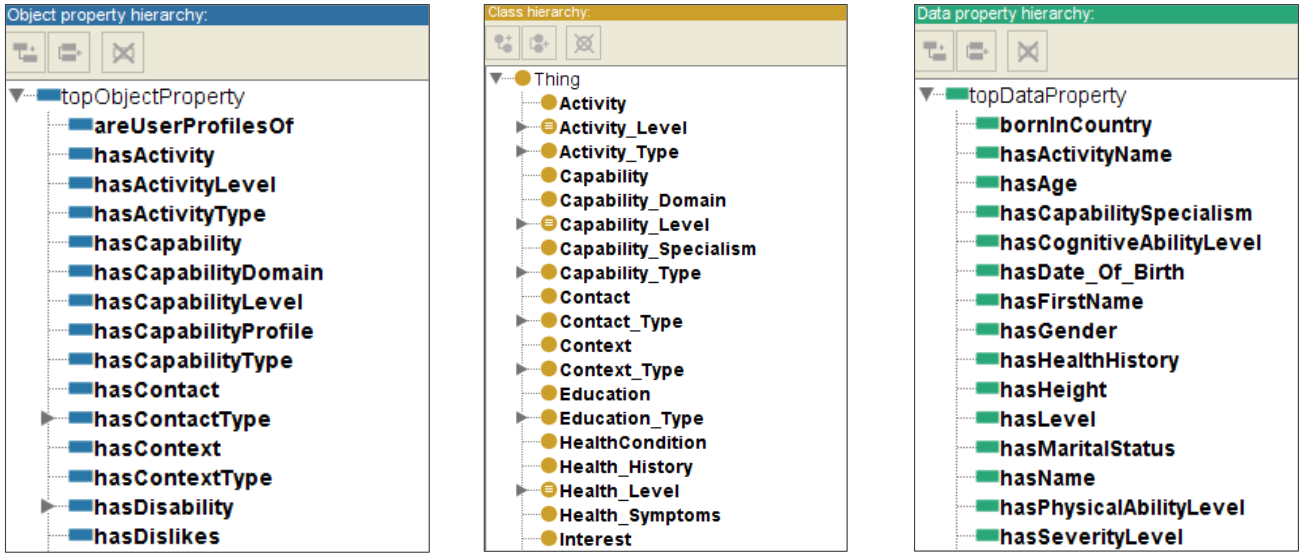
\includegraphics[width=0.70\textwidth]{skillen_ontology.png}
\caption{An overview of the User Profile Ontology classes, object properties and 
data properties~\citep{skillen2012ontological}.}
\label{fig:skillen_ontology}
\end{figure}

\subsubsection{Generic User Modelling Systems}
\label{sec:generic_users}

Apart from the analysed models there is another generic approach for modelling 
users known as Shell Systems. More focused in the field of \ac{ai}, these 
solutions consider the user model as a source of information which are built on 
assumptions about relevant user aspects or 
behaviour~\citep{pohl_logic_based_1999}.

\citet{heckmann_ubiquitous_2005} differentiates between the model, which is where 
the user data is collected, and the modelling system, which is the module that
manages the model. Besides, he remarks the following two definitions
from~\citet{wahlster_user_1989} previous work:

\begin{description}
  \item[\Defi{User Model (I), by~\citet{heckmann_ubiquitous_2005}}] \hfill \\
  \begin{mdframed}[hidealllines=true,backgroundcolor=gray!20]
  \textit{``A user model is a knowledge source in a system which contains explicit
  assumptions on all aspects of the user that may be relevant to the behaviour
  of the system. These assumptions must be separable by the system from the
  rest of the system's knowledge''}~\citep{wahlster_user_1989}.
  \end{mdframed}

  \item[\Defi{User Model (II), by~\citet{heckmann_ubiquitous_2005}}] \hfill \\
  \begin{mdframed}[hidealllines=true,backgroundcolor=gray!20]
  \textit{``A user modelling component is that part of a system whose function is to
  incrementally construct a user model; to store, update and delete entries;
  to maintain the consistency of the model; and to supply other components of
  the system with assumptions about the user''}~\citep{wahlster_user_1989}.
  \end{mdframed}
  
\end{description}


% % \begin{framed}
%   \begin{mydef}
%     {A user model is a knowledge source in a system which contains explicit
%     assumptions on all aspects of the user that may be relevant to the behaviour
%     of the system. These assumptions must be separable by the system from the
%     rest of the system's knowledge.~\citep{wahlster_user_1989}}
%   \end{mydef} 
% % \end{framed}
% 
% % \begin{framed}
%   \begin{mydef}
%     {A user modelling component is that part of a system whose function is to
%     incrementally construct a user model; to store, update and delete entries;
%     to maintain the consistency of the model; and to supply other components of
%     the system with assumptions about the user.~\citep{wahlster_user_1989}}
%   \end{mydef} 
% % \end{framed}

Assumptions are deeply studied and depicted in~\citep{pohl_logic_based_1999}. 
In this section, a quick overview of how these systems behave is performed to 
just take into account the difference between generic user modelling approach 
(user modelling shells) and the approach followed in this dissertation, which 
is related to Human-Computer Interaction.

In 1986 \ac{gums} is presented. This software allowed developers to make 
user-adaptive applications by defining several stereotypes, facts and rules to 
reason with~\citep{finin_gums_1986}. \acs{gums} supports the addition of new 
facts in runtime, manages facts inconsistencies and answers the application 
about assumptions about the user~\citep{kobsa_generic_2001}. The following 
systems are several examples of generic user systems developed in the following 
years (chronological ordered):

\begin{itemize}
  \item DOPPELGÄNGER, which uses several learning techniques for generalizing
  and extrapolating sensor data for the development of the user model
  \citep{orwant_doppelgangeruser_1991}.
  \item \ac{umt}, which supports the definition of hierarchically ordered 
  stereotypes about the user, rules for user model inferences and contradiction 
  detection~\citep{brajnik1994shell}.
  \item TAGUS, which uses first-order formulas to represent assumptions about
  the user~\citep{paiva1994tagus}.
  \item The um toolkit, which models not only assumptions but beliefs, preferences and other
  user characteristics in attribute-value pairs~\citep{kay1994toolkit}.
  \item BGP-MS, which permits user and groups of users assumptions~\citep{kobsa1994user}.
\end{itemize}

% MÁS SISTEMAS? SOLO LLEGAMOS A 1995\dots ESTOS SISTEMAS SON MUY ANTIGUOS, SI NO PONEMOS A
% PARTIR DEL 2000 MEJOR NI PONERLOS IGUAL\dots


% A significant aspect of these systems is that they are required to be usable in
% as many applications as possible. This is, domain independent. Therefore, they
% are expected to provide as many services as possible. On the contrary, in Human-Interaction
% user modelling approaches this is, in fact, an issue \citep{cita_falta_modelos_usuarios_comparar}.
% This problem is addressed in Chapter~\ref{cha:el_que_sea}.

% Domain independence
% 
% Known systems: 
% 
% GroupLens
% LikeMinds
% Personalization Server
% Frontmind
% Learn Sesame

% \InsertFig{heckmann_model}{fig:heckmann_model}{Several user model property dimensions \citep{heckmann_user_2007}}{}{0.70}{}

% ----------------------------------------------------------------------



\subsection{Users Models Comparison}
\label{sec:user_model_comparison}

In this section we describe our user modelling requirements nurtured by the 
earlier works described. As mentioned before, there are several perspectives 
regarding the user modelling requirements. In this dissertation the \ac{hci} 
perspective is taken. This means, as~\citet{pohl_logic_based_1999} states, 
that the user model refers to user characteristics using a certain system (see 
Section~\ref{sec:chronological_review}). In Chapter~\ref{cha:ontology_model}
the AdaptUI models for user, context and device are described. These models
have been designed considering each of these entities as a set of characteristics
that define them. Hence, the adaptation platform is able to evaluate the
combination of these characteristics and perform the corresponding adaptation.
Thus, the \ac{hci} interpretation of user modelling suits the goal pursued
by AdaptUI.

% Now that the \ac{hci} viewpoint has been remarked, we emphasize the amount of 
% different domains that are addressed in the literature considering user 
% modelling. 

In the following lines the amount of different domains addressing user modelling 
are highlighted. From product design to multimedia and user interfaces adaptation, 
every approach follows the same purpose: to consider several user characteristics 
to improve the system and user's satisfaction and product or service usability. 
However, although these solutions share the same objectives, the considered 
characteristics differ a lot. For ubiquitous and more context-aware domains, 
activities are taken into account. For example,
~\citet{razmerita_ontology_based_2003} discuss an ontology based architecture, 
which aims to be generic by collecting user data through two different ways 
(explicitly and implicitly).~\citet{golemati_creating_2007} also take an 
ontological point of view to avoid the problem of domain dependency (among 
others) by designing a more general, comprehensive and extensible ontology. 

\citet{gauch_ontology_based_2003} remark in the presented ontology the 
importance of time. Regarding the studied domain (web browsing) time is 
significant because it might help characterizing the user considering the spent 
time reading an article or visiting a website. Well known and popular 
recommendation systems, as YouTube, utilise this information combined with 
different explicit and implicit sources from the user interaction to make proper
recommendations~\citep{davidson_youtube_2010}.

User activities have also been considered as relevant for many authors in the 
literature. The first example is the Doppelgänger 
system~\citep{orwant_doppelgangeruser_1991} (1991), which uses activities for 
sharing relevant user information to different applications. In the same 
way,~\citet{persad_characterising_2007},~\citet{heckmann_gumogeneral_2005}
and~\citet{skillen2012ontological} modelled activities to take user's behaviour
and interaction into account for the proposed classifications and systems. For
~\citet{hatala_ontology_based_2005} activities are also vital within 
context-aware environments.

As occurs with context modelling (see Section~\ref{sec:context_model_comparison})
many different techniques are available for the model representation. This usually
depends either on the developer, because of his/her experience, or in the system's
technical characteristics. For example, if the system is able to performs inference
with the user data an ontology based representation could be more helpful than
an object based one.~\citet{strang_context_2004} demonstrated that ontological
modelling is more appropriate for ubiquitous computing environments.

It is also common to model physiological related characteristics of the user.
For example, the works by~\citet{gregor_designing_2002} 
and~\citet{persad_characterising_2007} consider physical, cognitive an sensory 
capabilities.~\citet{skillen2012ontological} also model several user abilities 
for performing different tasks and activities. The problem is that being aware 
of these capabilities is difficult and, in some cases, poorly practical. For 
example, measuring the sight capability of one individual requires physiological 
experience or advice. Besides, people with the same affection do not respond in 
the same way. A person who was born blind would interact differently with the 
environment than another who has been losing sight during his/her life. The 
precise same disability (e.g., tunnel vision) might affect different people 
in many different ways depending on their personal skills (e.g., adaptability,
orientation, and so forth). This might lead to an idea. What if, instead of 
modelling physiological skills (disabilities), we were able to model user's 
capabilities? The first approximation for this is found 
in~\citet{casas_user_2008} work. \citeauthor{casas_user_2008} present a user 
profile which abstracts from physiological aspects and lets users manage and 
configure their own profile. On the contrary, \citet{skillen2012ontological} 
model user capabilities as a set of abilities which allow users to perform some 
task or activities. Although this perspective covers many user capabilities, it
still needs a deeper understanding of physiological user capabilities.

On the other hand,~\citet{fischer_user_2001} comments that it not only is 
difficult to model users because of the wide range of different types of people 
that exist. He also considers that each individual changes with experience and 
through time. For example, old people's capabilities decrease with ageing. This
idea is shared with~\citet{gregor_designing_2002}, whose work is centred around
the elderly. \citet{heckmann_ubiquitous_2005} not only considers that users 
might evolve (from an \ac{ai} perspective), but he also takes new context 
information from the inference process. This also opens a new point of view 
that we address in Section~\ref{sec:context_disabilities} and it is about taking 
context as a significant user's environment entity that might directly influence 
the user's capabilities. In other words, users change through experience, time 
and, in concrete situations, due to the current context characteristics. For 
example, an individual might not suffer from any mobility disability, but in a 
crowded street would be difficult to perform several daily activities (just 
walking could be difficult).~\citet{razmerita_ontology_based_2003} also address 
this issue when they talk about the implicit user information collecting 
process. This, of course, deals with the concept of dynamism.

\citet{evers_achieving_2012} consider that respecting user's interactive 
behaviour with applications needs to be taken into account. On the other hand,
~\citet{pereira_triple_2005} analyses the differences between emotional and
perceptional user characteristics. 

% Several authors have also noticed the importance of tolerating the management of
% non-trustworthy data. Ambiguity and uncertainty mean working with data which might
% not reflect the current situation. Beynon et al. considered uncertainty as an actual
% problem to deal with \citep{beynon2000dempster}.

Table~\ref{tbl:user_comparison} summarizes the analysed approaches for user
modelling, emphasizing the modelled user characteristics and domains. 


% Besides, 
% although in a first version every used technique was remarked, in this 
% dissertation we focus on remarking just those which follow an ontology-based 
% approach. This is because many of the cited works are more theoretical or 
% surveys, or they just give some advices about important context data when 
% facing a context modelling task. Besides, \citet{strang_context_2004} 
% demonstrate that using ontologies is more appropriate for modelling 
% context-aware systems.

\begin{table}
  \caption{Related work for the user modelling approaches. Under the user
 characteristics heading \underline{A}ctivities or behaviour, \underline{C}apabilities,
 \underline{Ex}perience,  \underline{I}nterests, \underline{E}motions,
 \underline{P}ersonal, \underline{S}tress and \underline{L}ocation information
 are presented.}
 \label{tbl:user_comparison}
\footnotesize
\centering
 \begin{tabular}{l c c c c c c c c c}
  \hline 
  \textbf{Solution} & \textbf{Ontologies} & \multicolumn{8}{c}{\textbf{User characteristics}}\\
  \textbf{(Domain)} & & \textbf{A} & \textbf{C} & \textbf{Ex} & \textbf{I} & \textbf{E} & \textbf{P} & \textbf{S} & \textbf{L} \\
  \hline
  
  2002,~\citet{gregor_designing_2002}		&  		& & $\checkmark$ & $\checkmark$ & & & & & \\
  (Inclusive design)\\
  2003,~\citet{gauch_ontology_based_2003}	& $\checkmark$	& & & & $\checkmark$ & & & &\\
  (Automatic profiling)\\ 
  2003,~\citet{razmerita_ontology_based_2003}	& $\checkmark$	& $\checkmark$ & & & $\checkmark$ & & $\checkmark$ & & \\
  (\ac{kms})\\				
  2005,~\citet{hatala_ontology_based_2005} 	& $\checkmark$ 	& & & & $\checkmark$ & & $\checkmark$ & & $\checkmark$ \\
  (Tangible interfaces)\\		
  2005,~\citet{pereira_triple_2005} 		& 		& & & & & $\checkmark$ & & &  \\
  (Multimedia adaptation)\\
  2007,~\citet{persad_characterising_2007} 	&   		& $\checkmark$ & $\checkmark$ & & & & & & \\
  (Product design demands)\\
  2007,~\citet{golemati_creating_2007} 		&  $\checkmark$   	& $\checkmark$ & & $\checkmark$ & $\checkmark$ & & $\checkmark$ & & \\
  (User profiling)\\
  2007,~\citet{heckmann_gumogeneral_2005} 	& $\checkmark$   	& $\checkmark$ & & & & $\checkmark$ & $\checkmark$ & $\checkmark$ & \\
  (Ubiquitous applications)\\
  2008,~\citet{casas_user_2008} 		&  		& & $\checkmark$ & $\checkmark$ & & & & & \\
  (\ac{aui}\\
  2012,~\citet{evers_achieving_2012} 		&  		& & & & & & & $\checkmark$ & \\
  (Adaptive applications)\\
  2012,~\citet{skillen2012ontological} 		&  $\checkmark$	& $\checkmark$ & $\checkmark$ & & $\checkmark$ & & & & $\checkmark$ \\
  (Mobile environments)\\
  \hline

\end{tabular}
\end{table}


